With the PEGylation process fully optimized, we took the first step towards immunolabeling a full 3D artificial cornea, namely immunolabeling of a monolayer of cells on a microscope coverslip. The cells used were human dermal fibroblasts (HDFs) that express $\alpha5\beta1$-integrin, the same surface protein that we are targeting on the corneal cells. Performing immunolabeling on the monolayer allows assessment of the efficacy of the indirect immunolabeling process only, disregarding the collagen and removing the financial and temporal costs of building a complete corneal construct.

\section{Structure of the Immunolabeling Experiment}
\label{structureoftheimmunolabelingexperiment}

Several different preparations of cells were used to determine the efficacy of the immunolabeling process. Each of them adds one or more key components of the process, which should yield very little increase in the scattering contrast until the full labeling system is assembled. The 6 preparations and their expected outcomes are described in \autoref{tab:6MarchPrepTable}.

The cells were prepared according to the procedure found in \autoref{The6MarchImmunolabelingProtocol}; in brief, the procedure is

\begin{enumerate}
\item Fix cells with paraformaldehyde

\item Permeabilize with Triton-X

\item Label the nuclei with Sytox Green and the actin filaments with phalloidin (fluorescent stains); simultaneously perform immunoblocking with goat serum.

\item Add primary antibody if appropriate for a given preparation

\item Add secondary labeler (if any)

\end{enumerate}

In between each stage, the sample is washed to remove residues of the previously applied label. Each preparation had three different samples (except for the 2Au preparation, which unfortunately had only two) to minimize intrinsic variation during inter-preparation comparison. After labeling, each sample was imaged in three different places with the confocal microscope, using both fluorescence and backscattering modes, and then each sample was imaged at five different $500\,\mu\mathrm{m}\,\times\,500\,\mu\mathrm{m}$ field of view locations with the OCM (except for 2Au, for which each sample was sampled at 10 different locations).

\rowcolors{1}{}{lightgray} 
\begin{table}[hb]
\caption{Description of the six preparations used in the 6 March immunolabeling experiment; each preparation is described by whether the primary antibody (MAB1999) was added, what secondary labeler (AP124F, AP124F PEGylated to Au nanospheres, or naked Au nanospheres) was added, and whether or not an increase was expected in backscattering or fluorescence.}
\begin{minipage}{\linewidth}
\setlength{\tymax}{0.5\linewidth}
\centering
\small
\begin{tabular}{lp{2cm}p{2cm}p{2cm}p{2cm}} \toprule
Preparation Name&Primary Antibody?&Secondary Labeler?&+Scattering Expected?&+Fluorescence Expected?\\
\midrule
Cells Only&No&No&No&No\\
2 only&No&Secondary Ab&No&No\\
1--2&Yes&Secondary Ab&No&Yes\\
2Au&No&OPAb-Au-PS&No&No\\
1--2Au&Yes&OPAb-Au-PS&Yes&Yes\\
Au&No&Naked Au&Yes but non-specific&No\\

\bottomrule

\end{tabular}
\end{minipage}
\label{tab:6MarchPrepTable}
\end{table}

The first preparation is just cells, grown on a coverslip. In the confocal microscope, a Zeiss LSM 510, we expect to see green fluorescence in the shape of the nuclei from the Sytox Green and red fluorescence in the shape of the actin filaments within the cell from the phalloidin. In the OCM, we expect to see backscatter contrast between the cells and the coverslip; however, the amount of backscattering from the cells should be quite low.

The next preparation is cells with the addition of only the secondary antibody, AP124F. The F in the AP124F signifies the presence of a fluorescent marker, specifically a fFluorescein isothiocyanate (FITC) molecule which has an emission spectrum peak at 521 nm. Since the AP124F binds specifically to the MAB1999, and no MAB1999 is present on the surface of the cells, all of the AP124F should be washed off. As a result, the 2 only preparation should be identical to the cells only preparation.

The 1-2 preparation, in contrast, has MAB1999 present. The MAB1999 should bind to the integrins on the surface of the cell, and the AP124F should bind to the MAB1999 in turn. This should manifest itself in the confocal microscope as fluorescence signal at 521 nm. The fluorescence should be localized to the integrins, which are situated in streaks at the edges of the cell. As the AP124F and MAB1999 do not increase the backscattering, the OCM images of the 1-2 preparation should be equivalent to the images of unlabeled cells.

The 2Au preparation should behave just like the 2 only preparation: the lack of MAB1999 should mean that the OPAb-Au-PS spheres cannot bind to anything, and should be washed off. This should result in confocal and OCM images equivalent to those of unlabeled cells.

The 1-2Au preparation should show fluorescence in the pattern of integrins for the same reason as the 1-2 preparation. In addition, the 1-2Au preparation should have gold nanoparticles localized to the integrins, increasing the backscattering signal observed in the OCM.

The naked Au nanospheres have no fluorescent marker, so an increase in fluorescence cannot occur. A scattering increase is expected from the application of the naked Au; however, as the naked spheres have no specific binding mechanism, their binding will not be localized. Instead, the naked Au spheres will likely bind to the coverslip and cells in a homogenous manner through van der Waals forces.

Together, these preparations serve as a set of controls. In the event that the 1-2Au system fails to show any scattering contrast increase, the 2 only and 1-2 only can be used to demonstrate that the AP124F does specifically bind to the MAB1999. This converse is also true: if the 2 only (or 2Au only) show increases in fluorescence or scattering, non-specific binding is occurring, indicating that some part of the PEGylation or labeling process is faulty.

\section{Results of the Immunolabeling Experiment}
\label{resultsoftheimmunolabelingexperiment}

\begin{figure}[p]
\centering
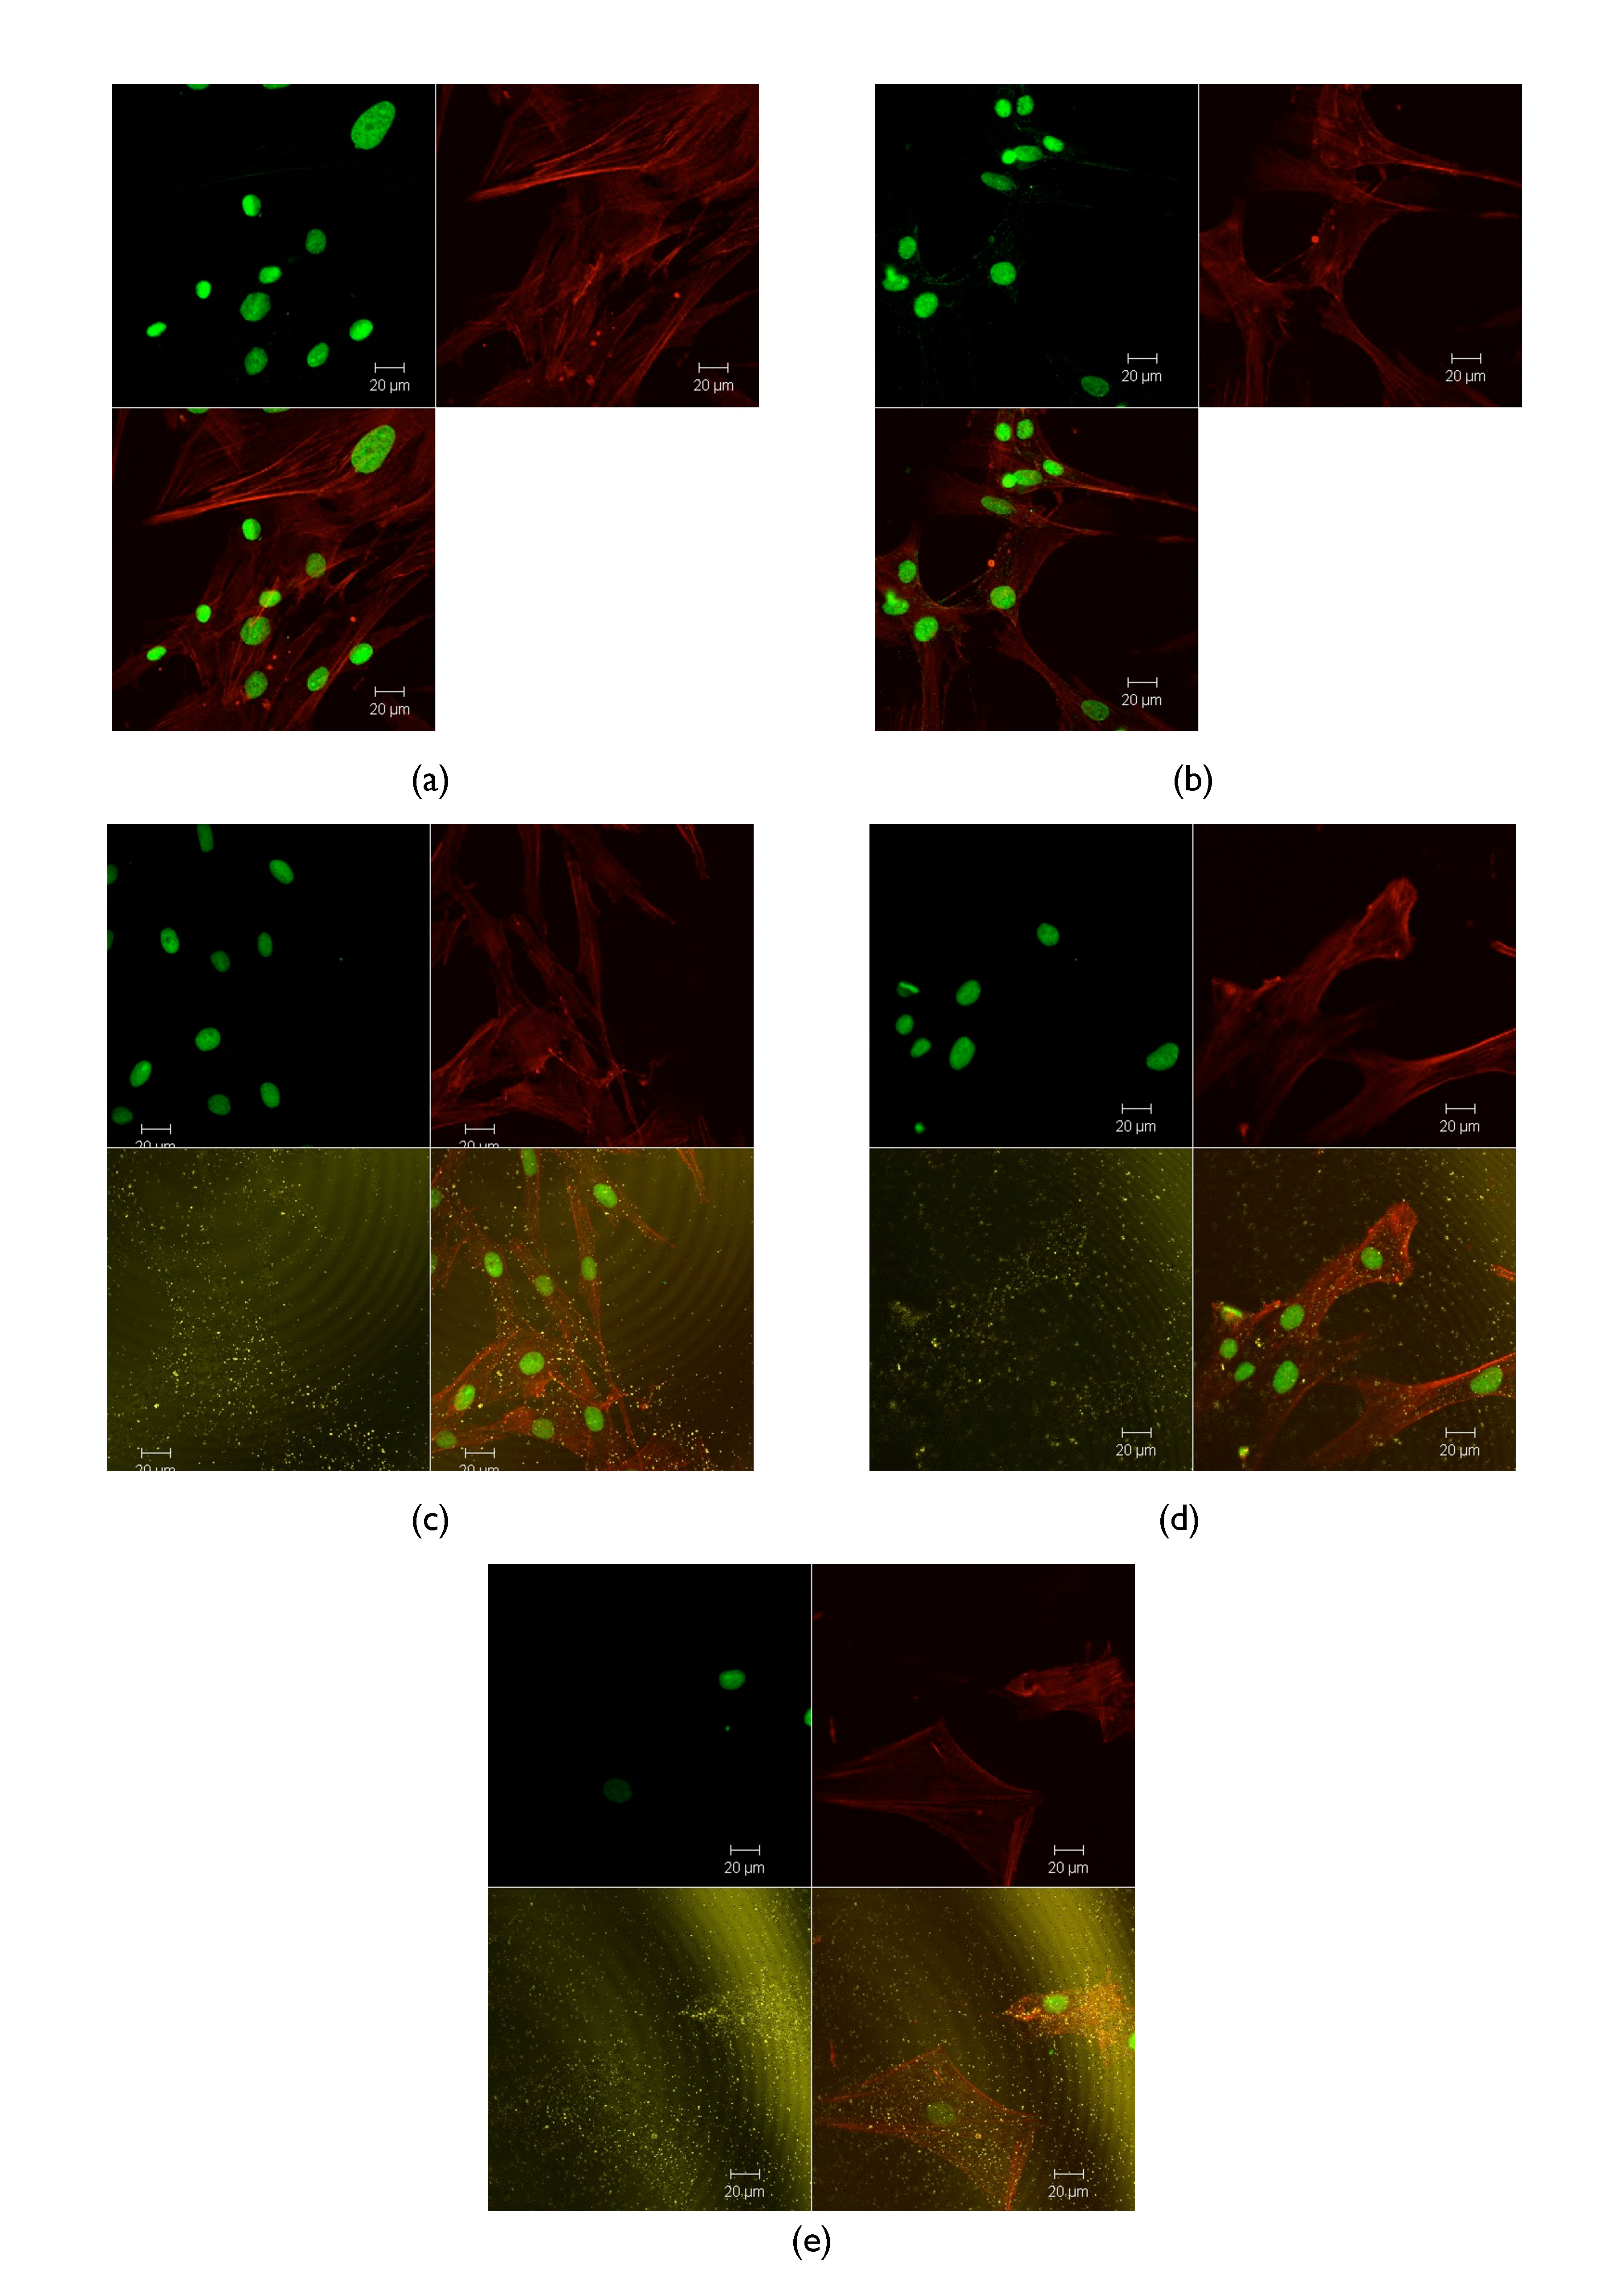
\includegraphics[keepaspectratio,width=\textwidth,height=9in]{ConfocalReps.pdf}
\caption{Confocal images of labeled preparations. Each image is a split view, showing Sytox and AP124F fluorescence (top left), phalloidin fluorescence (top right), backscattered light (c--e only; bottom left), and the composite view (bottom left, a and b; bottom right, c--e). Images correspond to preparations: (a) 2 only; (b) 1--2; (c) 1--2Au; (d) 2Au; (e) Au.}
\label{confocalcollage}
\end{figure}

\begin{figure}[p]
\centering
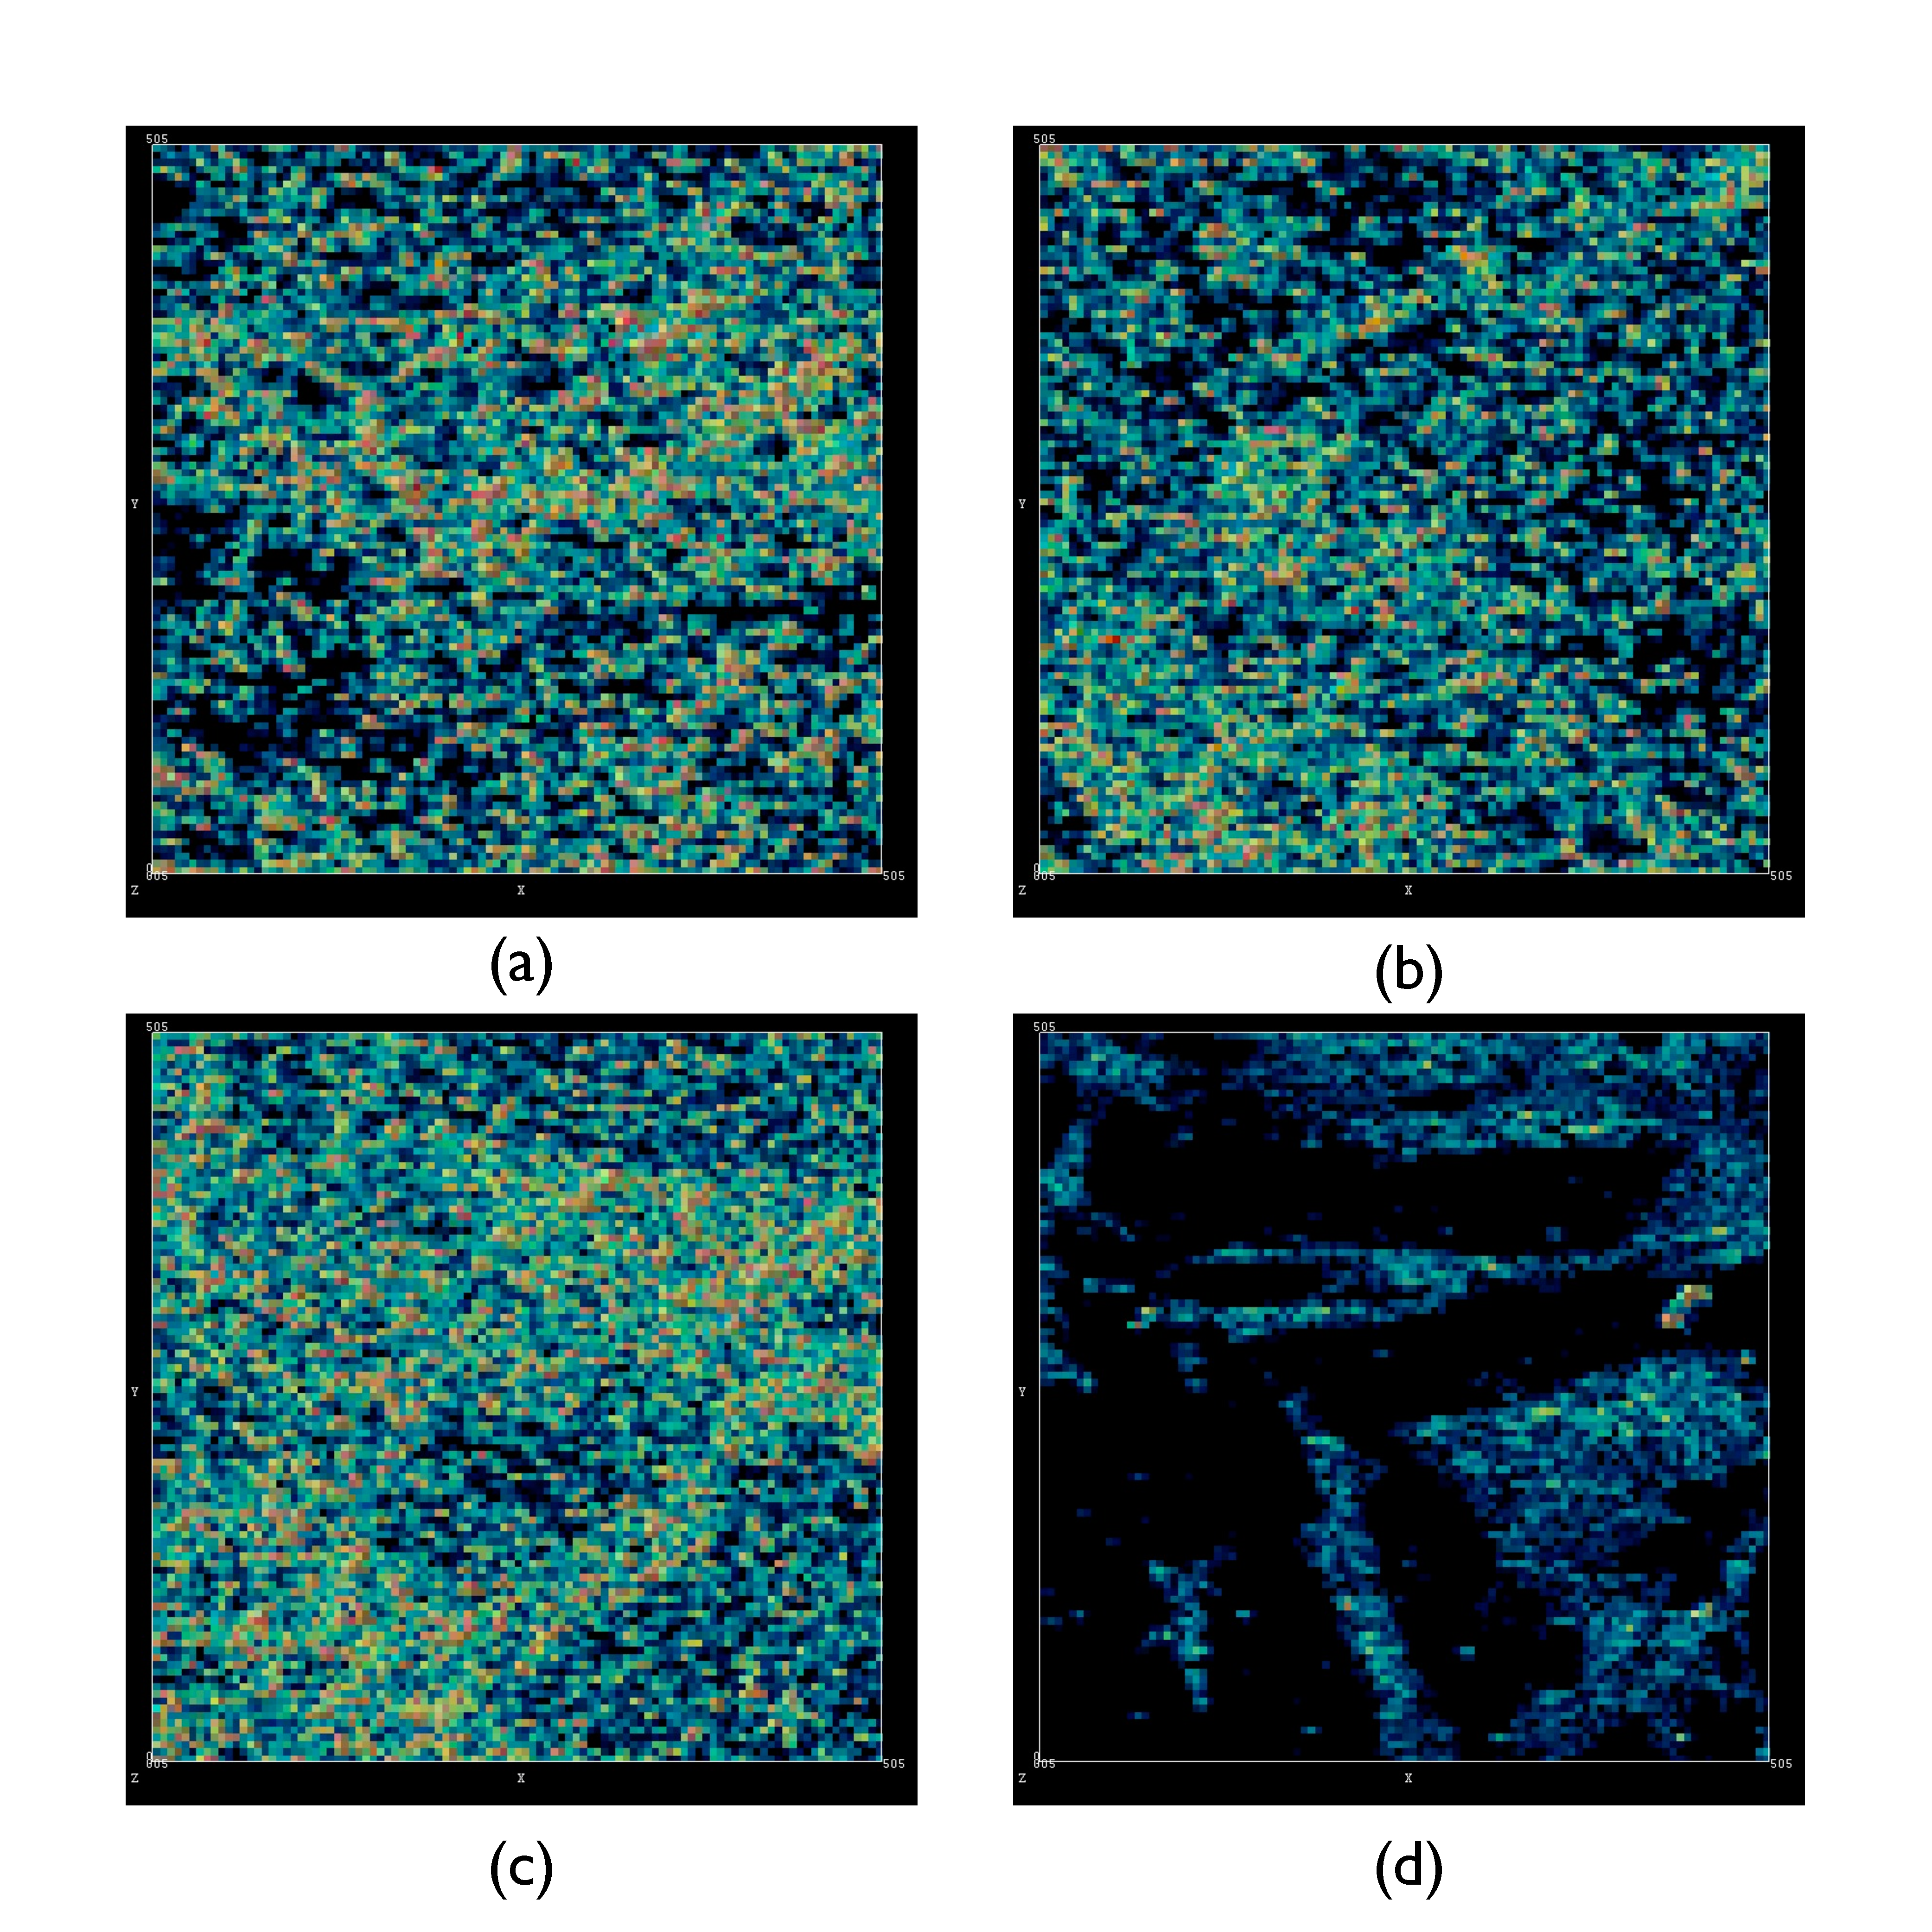
\includegraphics[keepaspectratio,width=\textwidth,height=0.75\textheight]{6marocmreprimages.pdf}
\caption{OCM images of labeled preparations. Images correspond to preparations: (a) 1--2Au; (b) 2Au; (c) Au; (d) Cells only.}
\label{marocmcollage}
\end{figure}

Representative confocal images for each labeled sample are shown in \autoref{confocalcollage}. Examining the between the 2 only and 1--2 confocal images reveals trails of green dots away from the nucleus only in the 1--2 sample; this is the expected pattern of labeled integrins. The appearance of stained integrins in only the 1--2 preparation indicates that both the primary and secondary antibodies bind only to the integrin and primary antibody, respectively. The samples with gold, however, are not as encouraging. Appearance of distinguishable cellular features in the back-reflectance channel indicates that the gold spheres bind to the cells--and to the coverslip--regardless of the presence of either the primary or secondary antibody. Nevertheless, cellular features are more easily distinguished in the 2Au samples, and most easily in the 1--2Au sample. This seems to indicate that some specific binding is occurring, but that a large amount of nonspecific binding is occurring as well.

Representative OCM images for the preparations labeled with gold as well as unlabeled cells are shown in \autoref{marocmcollage}. Clearly, all three gold-labeled preparations show a significant increase in scattering compared to the unlabeled cells. However, as in the confocal images, the Au and 2Au preparations show a strong increase in scattering, and allow for cellular features to be distinguished. Also correlated with the confocal images is the ease with which cellular features can be distinguished: the images from the Au preparation all have a very strong homogenous background, making it harder to discern the features, and in general the cellular features of the 1--2Au more easily distinguishable than those of the 2Au.

\begin{figure}[htb]
\centering
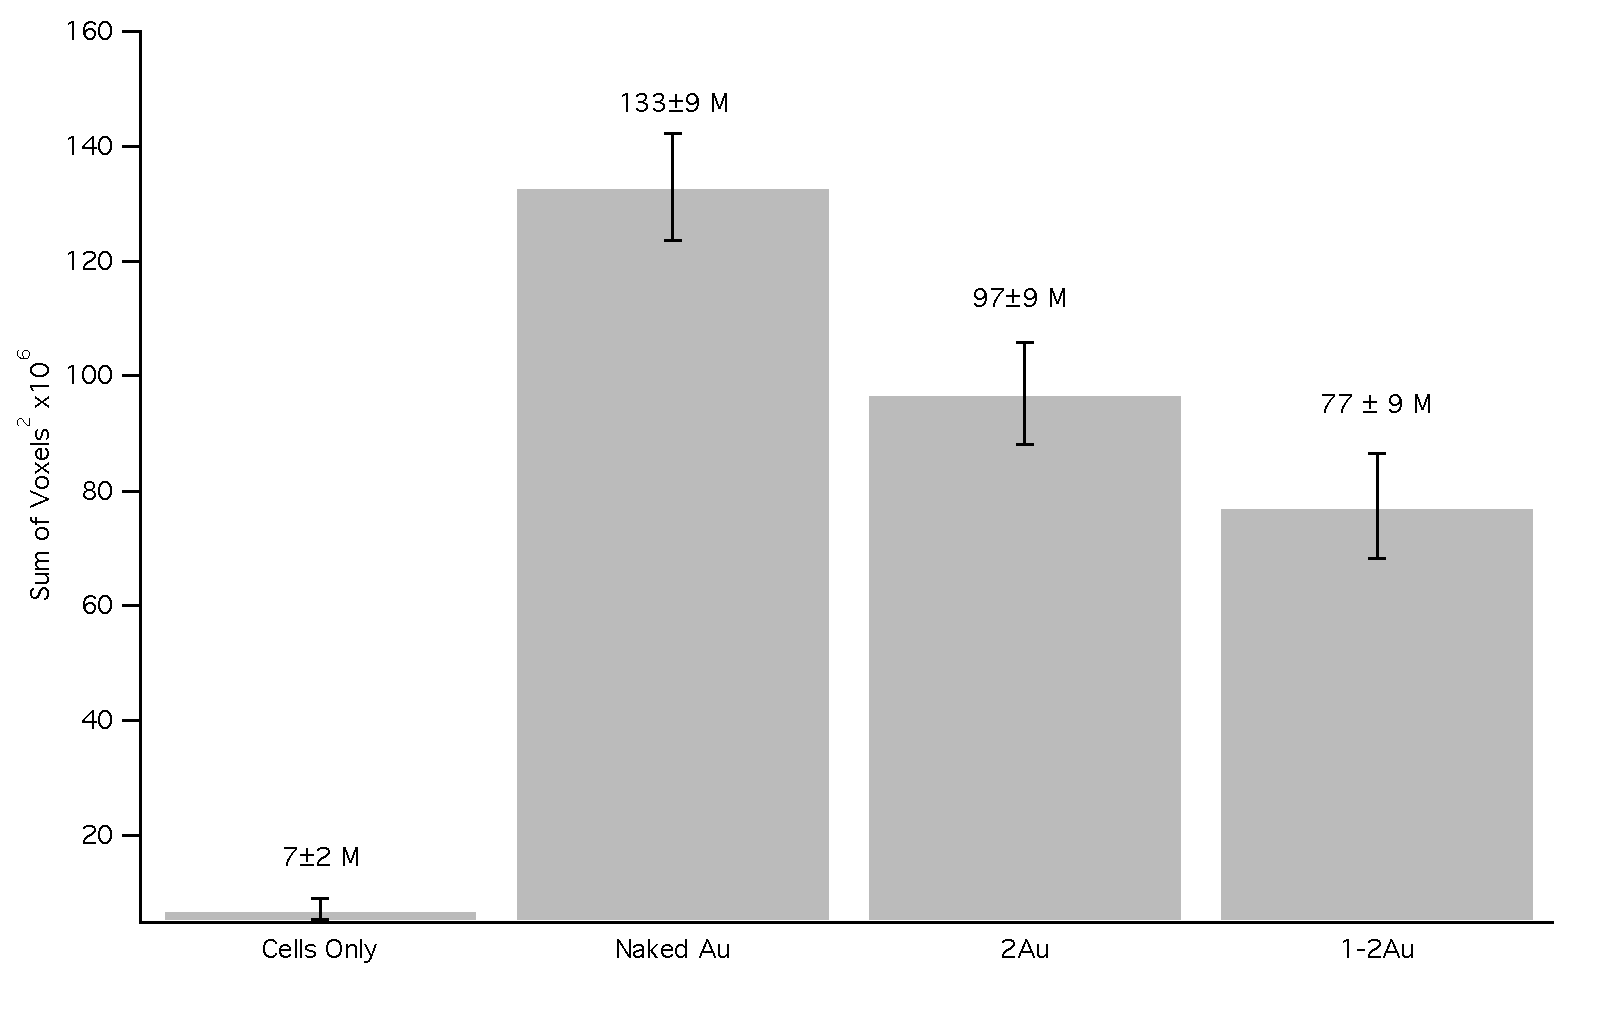
\includegraphics[keepaspectratio,width=\textwidth,height=0.75\textheight]{6marSOSgraph.pdf}
\caption{Sum of OCM voxel values squared for gold-labeled preparations and unlabeled cells; the sum of voxel values squared is a measure of the amount of backscattering from the field of view. Values are formed by taking the mean and standard error of sum of voxel values squared for each image corresponding to a given preparation.}
\label{marsosgraph}
\end{figure}


To quantify the amount of scattering increase, the sum of squares of the values of each voxel was tabulated for each OCM image. The mean and standard error of all the images from a given preparation were then calculated; those results are shown in \autoref{marsosgraph}. The increase in scattering in all three gold-labeled samples is shown quantitatively by comparing their sum of voxel values squared to that of the unlabeled cells. Among the gold-labeled samples themselves, the amount of scattering increase was the opposite of expected: the Au had the most scattering, then 2Au, then 1--2Au. However, the 2Au and 1--2Au samples are statistically indistinguishable.

The high amount of nonspecific binding was puzzling, and two hypotheses were put forth to explain the results of the labeling experiment. One possibility is that all of the spheres, especially the naked Au, bound to the cells via van der Waals forces. Because the naked Au has no dielectric material (protein) separating it from whatever surface it comes in contact with, the strength of van der Waals forces will likely be much larger for the naked Au than for the 2Au. The second possibility concerns the use of Triton-X, a permeabilizing agent. Triton-X is used to permeabilize the cells so that the Sytox Green and phalloidin stains can diffuse inside the cell and stain the nucleus and actin cytoskeleton, respectively. As a result, it was possible that the pores created by permeabilization of the cells allowed Au and 2Au to diffuse into the cell, but once in the cell, the gold nanospheres could not be removed by the washing process, leading to nonspecific contrast enhancement from nanoparticles inside the cell rather than on its surface. Furthermore, noting the strong background in some of the OCM images, there was some concern regarding the binding of the nanospheres to the coverslip surface itself. These concerns (van der Waals, permeabilization, and coverslip binding) led to a second round of immunolabeling experiments being performed on 3 April.